% Filename: Results
% Last update: 
%    - created%
%
%%%%%%%%%%%%%%%%%%%%%%%%%%%%%%%%%%%%%%%%%%%%%%%%%%%%%%%%%%%%%%%%%%%%%%

\section{Results}
\label{sec:results}

All SCIRun networks used to generate results will be included in the open-source dataset for future use and editing.

\subsection{Segmentation}

In this project, a full, detailed head was segmented into different tissue layers to be able to create an inhomogeneous three-dimensional mesh. 

\begin{figure}[H]
\begin{center}
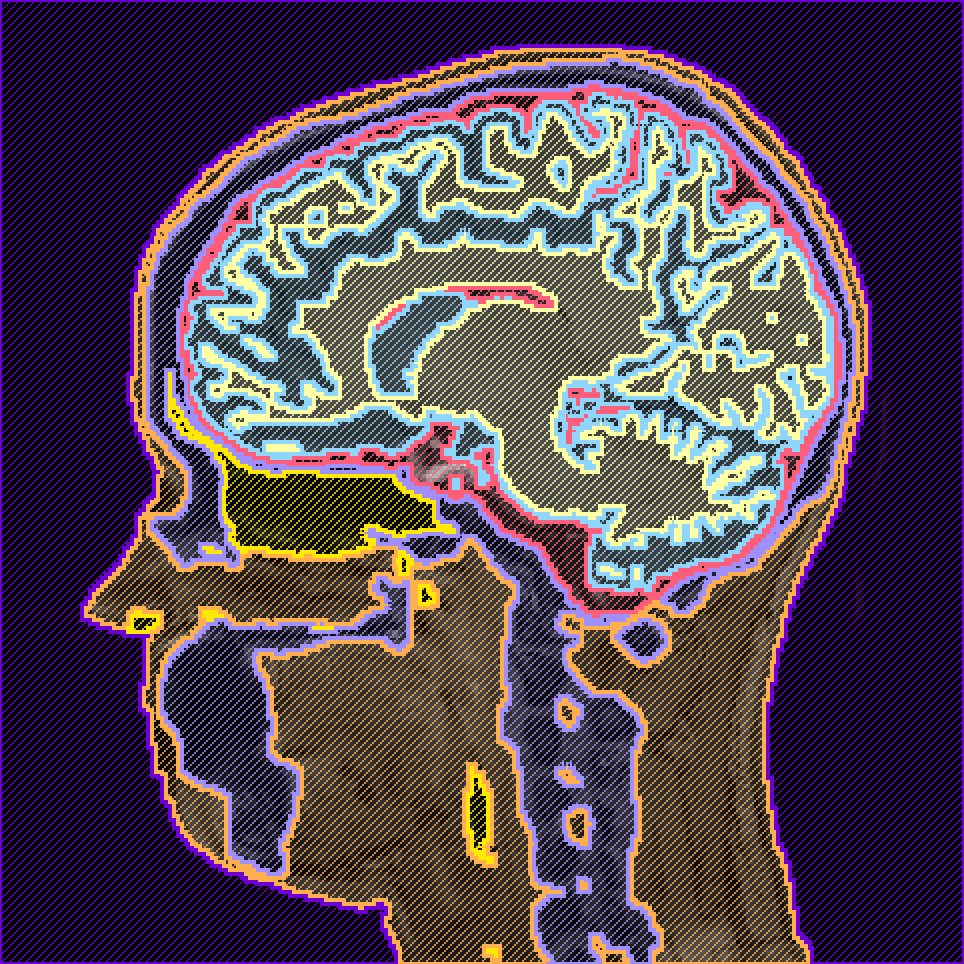
\includegraphics[height=2.35in]{Figures/seg_1}
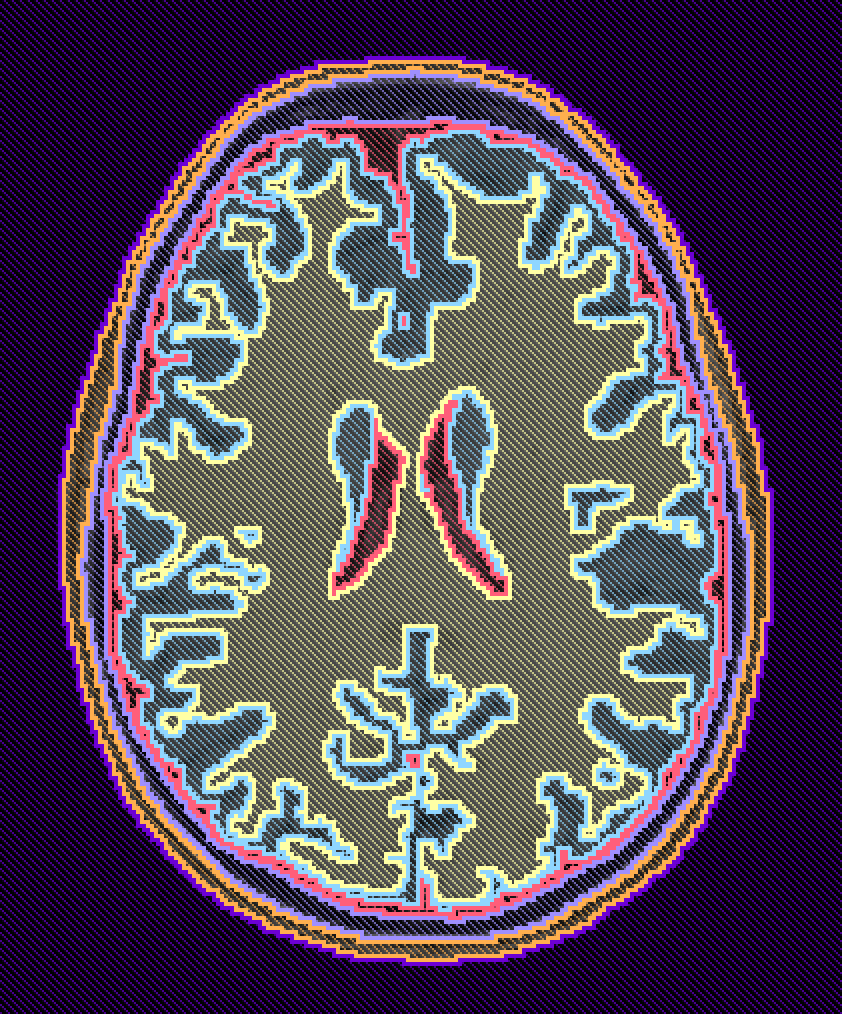
\includegraphics[height=2.35in]{Figures/seg_2}
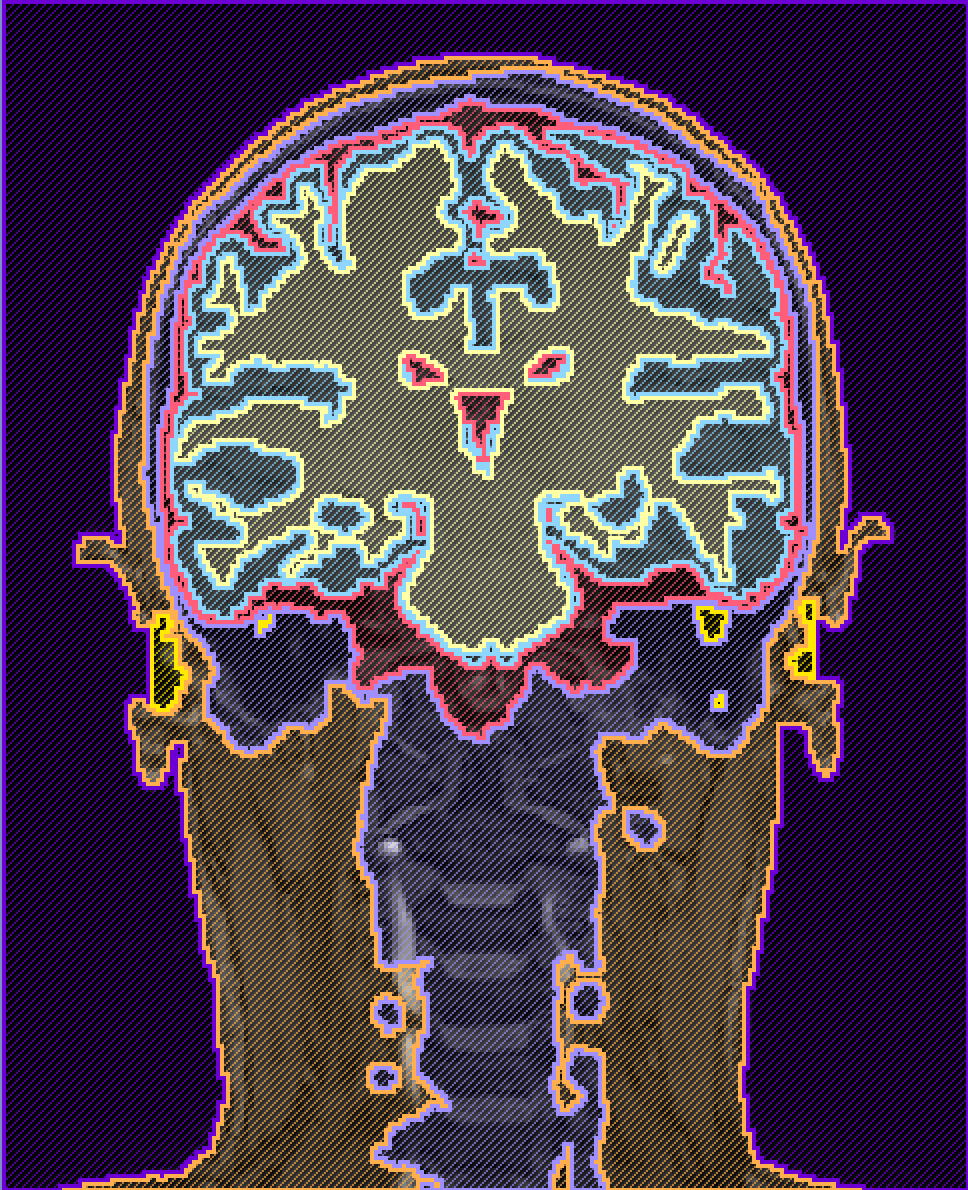
\includegraphics[height=2.35in]{Figures/seg_3}
\caption{A high-resolution, eight-layer full segmentation made with Seg3D }
\label{fig:fullseg}
\end{center}
\end{figure}

Since the dataset did not include a CT scan, the task of segmenting the skull and especially the sinus layers was daunting. A basic skull and bone layer was created using the FSL skull stripping feature  \cite{ref:bet2} in the brain extraction tool. This layer was then concatenated with a rough bone segmentation using thresholding in Seg3D of black pixels and manually correcting the segmentation. Although there was a rough skull/bone segmentation, the sinus segmentation was going to have to be made manually.

After receiving the pseudo-CT scan, skull/bone and sinus segmentations fit the brain segmentation well and had no artifacts from combining two different layers together, although the teeth are solid bone from the subject's permanent retainer.

\begin{figure}[H]
\begin{center}
\includegraphics[width=.49\textwidth]{Figures/skull_before}
\includegraphics[width=.49\textwidth]{Figures/skull_after}
\caption{Skull segmentation comparison: Made with BET \textit{(left)} and made with pseudo-CT \textit{(right). Segmentation was made using Seg3D.}}
\label{fig:skull}
\end{center}
\end{figure}

\begin{figure}[H]
\begin{center}
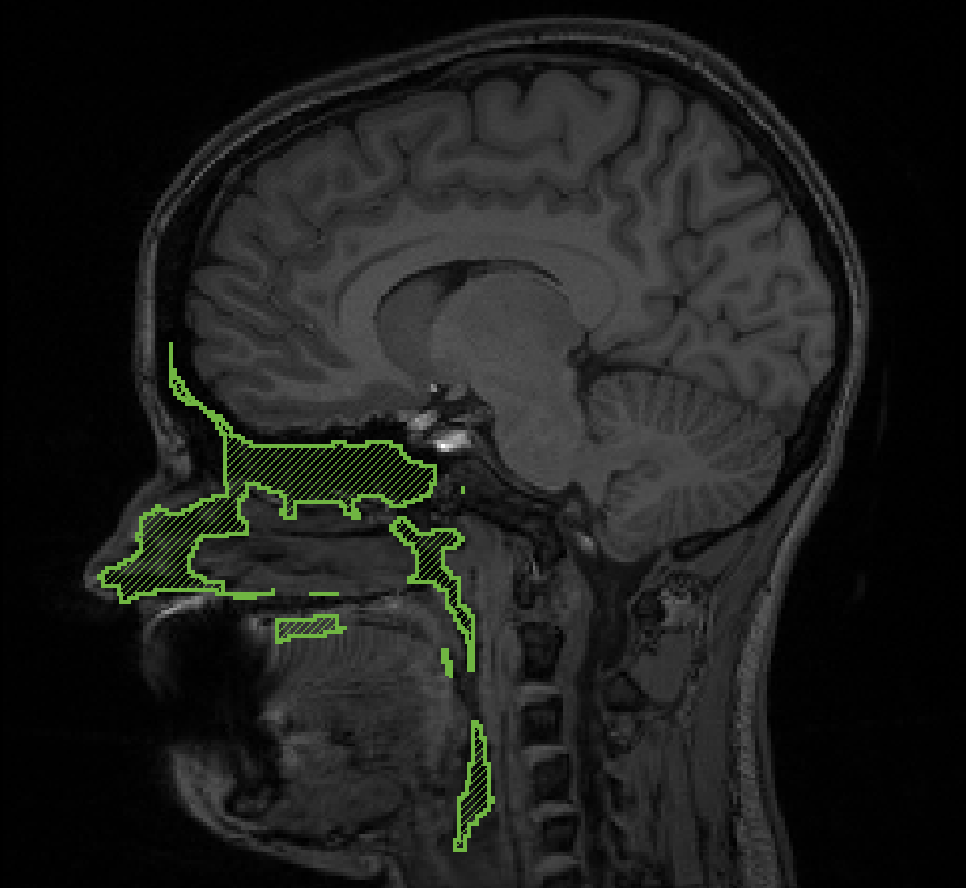
\includegraphics[width=.49\textwidth]{Figures/sinus_sag}
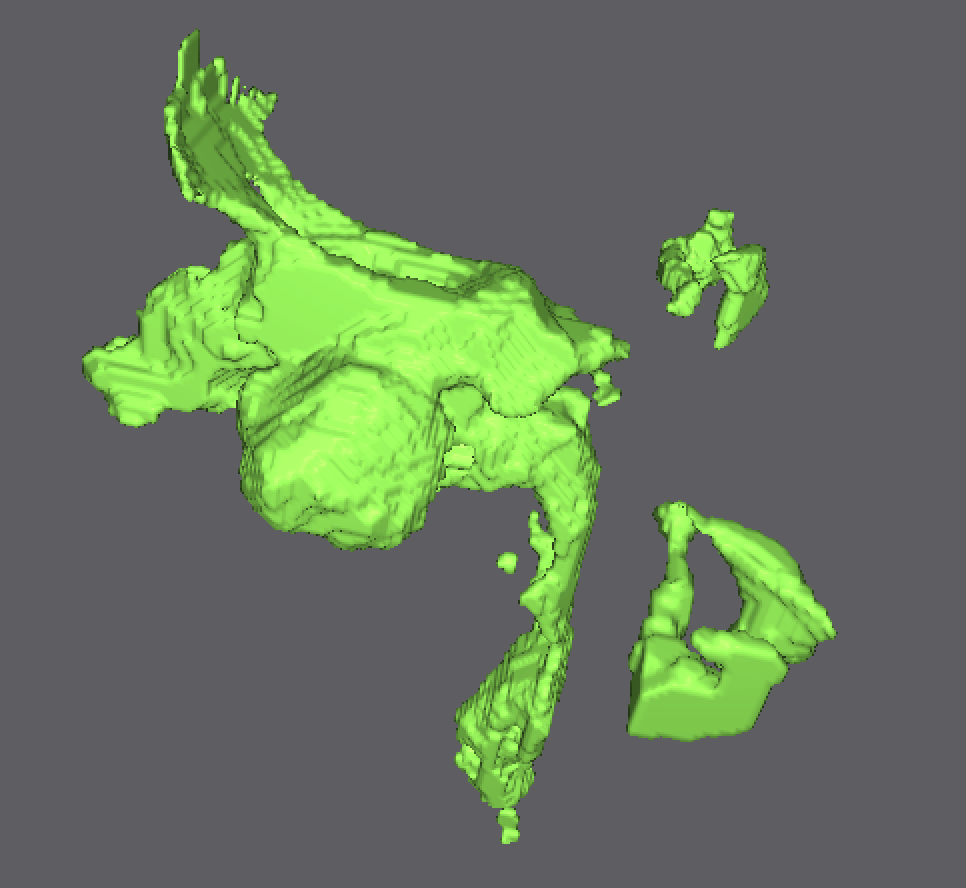
\includegraphics[width=.49\textwidth]{Figures/sinus_iso}
\caption{Sinus segmentation made using Seg3D}
\label{fig:sinus}
\end{center}
\end{figure}

When imaging, the subject was on her back which shifts the brain to the back of the head, resulting in thin segmented layers on the back of the head. There were also thin layers on the side of the subject's head, the bridge of the nose, and the bottom of the chin. These thin layers were made to be at least two pixels thick to ensure a mesh without holes.

\begin{figure}[H]
\begin{center}
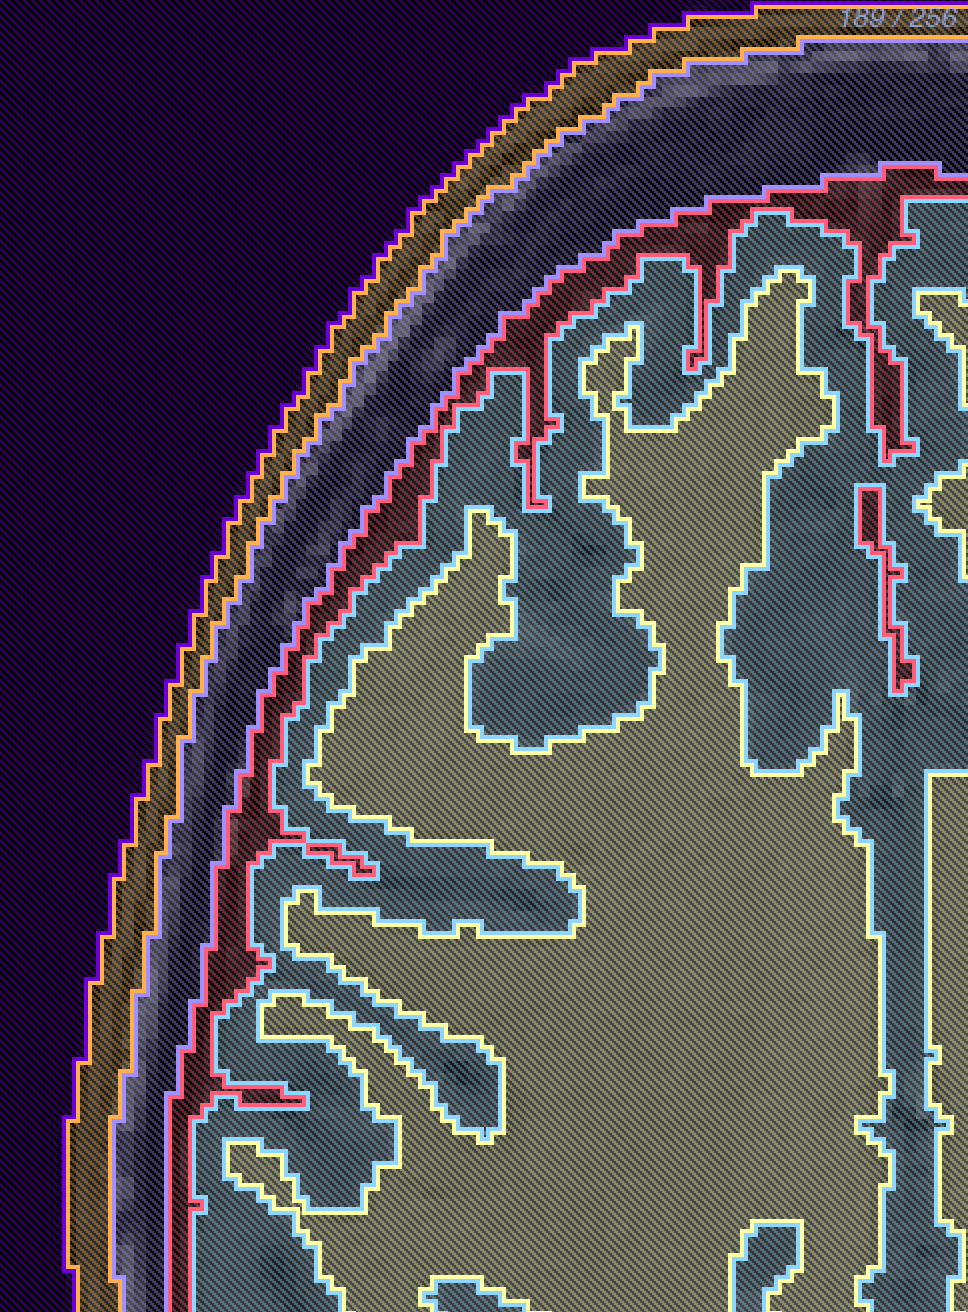
\includegraphics[width=.32\textwidth]{Figures/thin_layer_side}
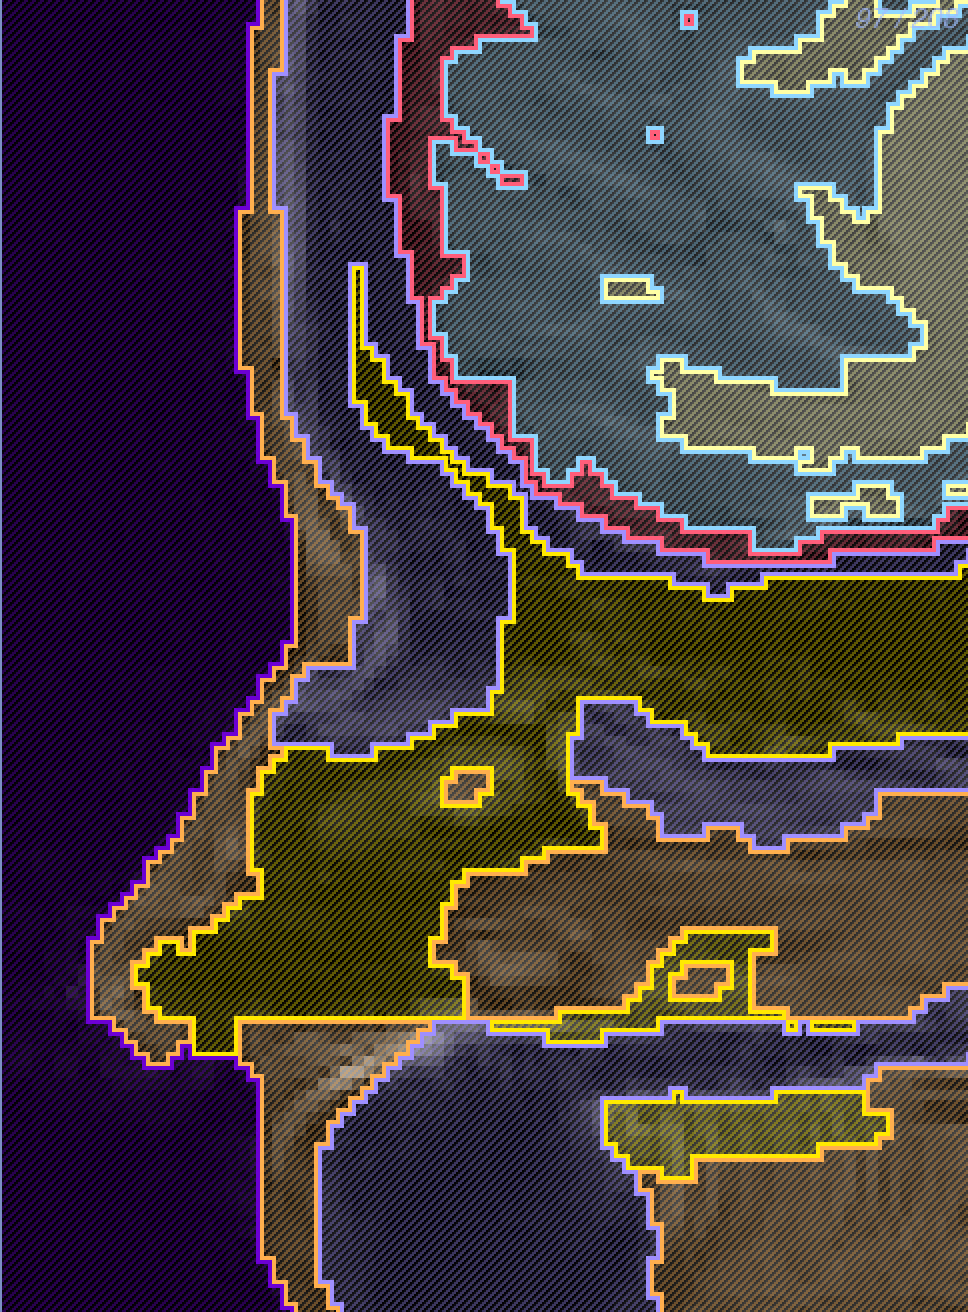
\includegraphics[width=.32\textwidth]{Figures/thin_layer_nose}
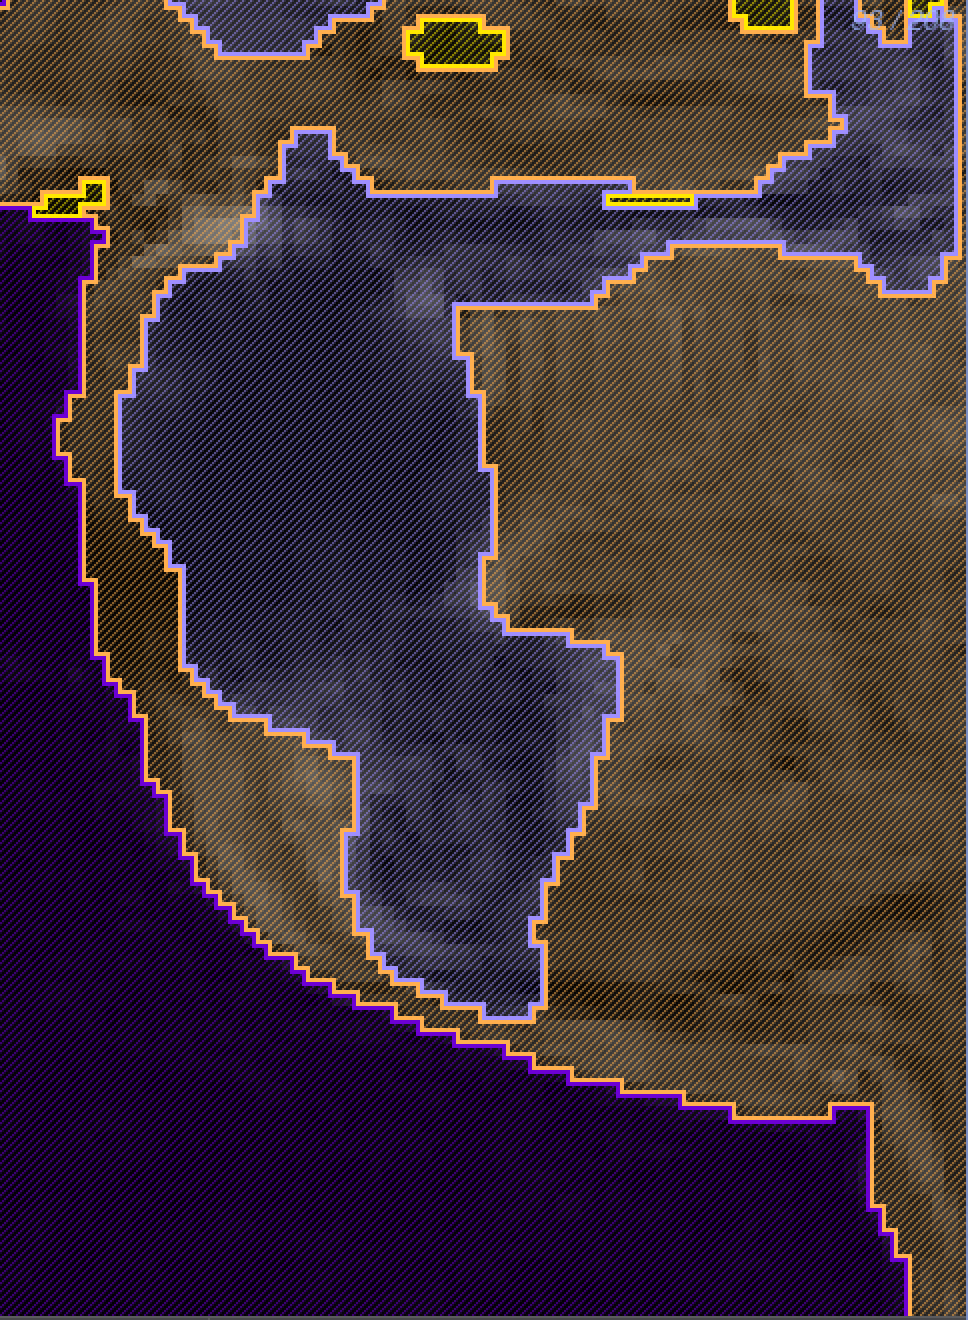
\includegraphics[width=.32\textwidth]{Figures/thin_layer_chin}
\caption{Thin layer segmentations: side of the head \textit{(left)}, bridge of the nose \textit{(middle)}, bottom of the chin \textit{(right)}}
\label{fig:thinseg}
\end{center}
\end{figure}

\subsection{Finite Element Meshes}

The highest resolution mesh, which was made with settings in Section \ref{sec:mesh}, had 60.2 million elements and 10.3 million nodes. This mesh was so large due to the complexity of the segmentation. Simulations run very slow when using this mesh due to its size, and required at least 32GB of RAM in order to not crash SCIRun. 

\begin{figure}[H]
\begin{center}
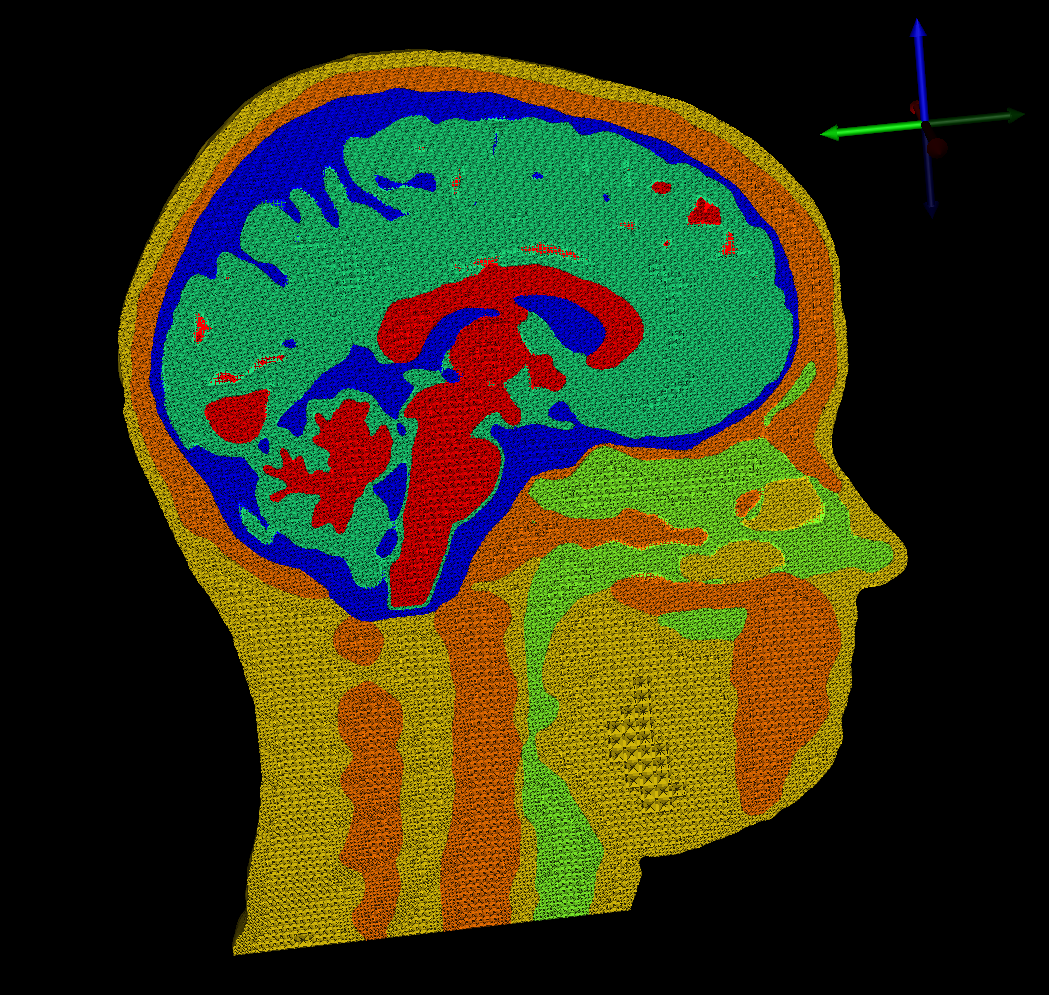
\includegraphics[width=.49\textwidth]{Figures/bigmesh_1}
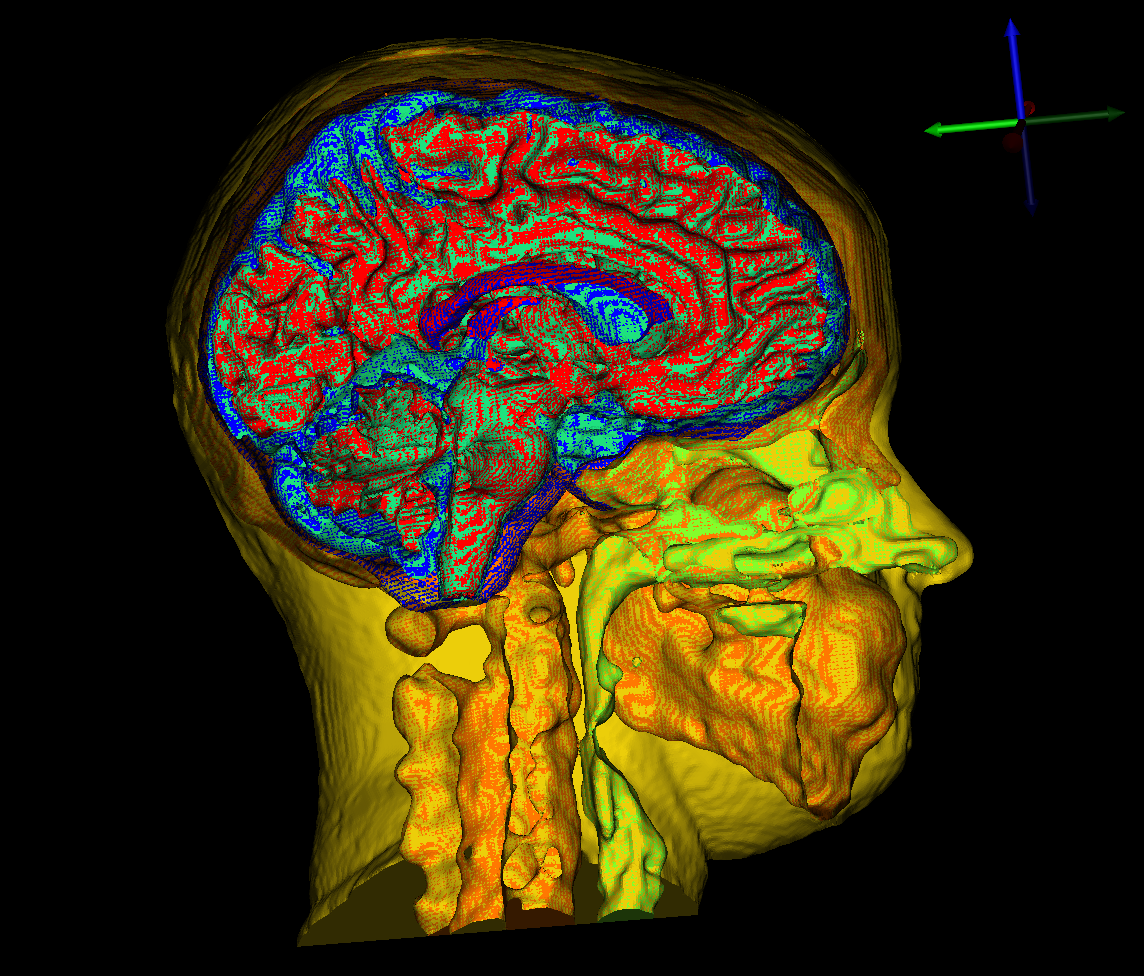
\includegraphics[width=.49\textwidth]{Figures/bigmesh_surface}
\caption{60.2 M element mesh: tetrahedral mesh \textit{(left)}, surface mesh \textit{(right)}}
\label{fig:bigmesh}
\end{center}
\end{figure}

Attempts were made to make smaller meshes in order to be able to run simulations more efficiently. After manually changing the sizing field as described in Section \ref{sec:mesh}, a mesh was produced with 15.7 million elements and 2.7 million nodes with no holes. However, this mesh contained one flat tetrahedra. It was later removed in a SCIRun network, and is currently being investigated by Cleaver software developers.

\begin{figure}[H]
\begin{center}
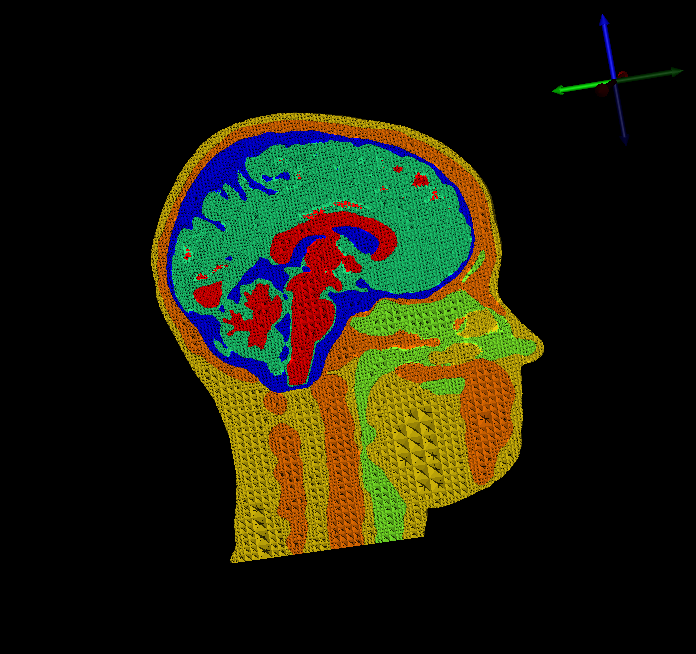
\includegraphics[width=.49\textwidth]{Figures/smallmesh_2}
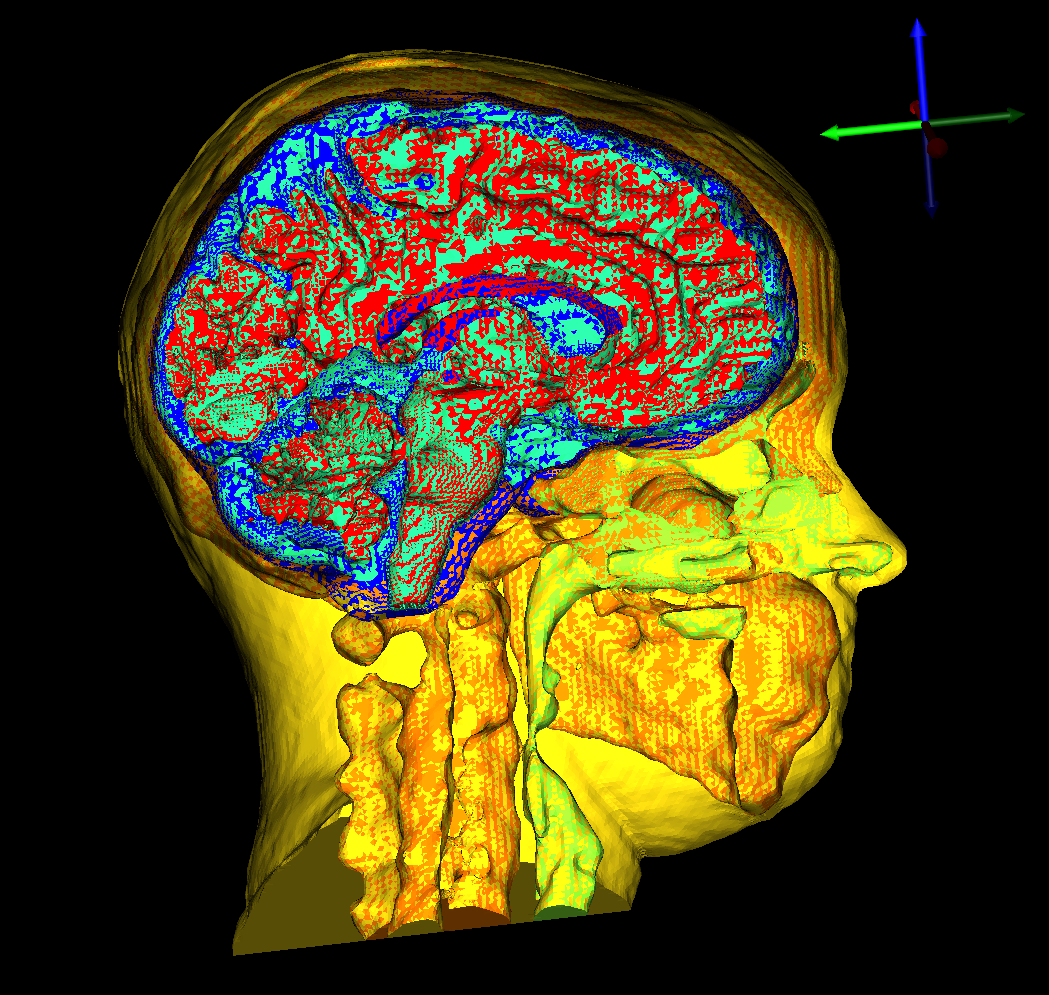
\includegraphics[width=.49\textwidth]{Figures/smallmesh_surface}
\caption{15.7 M element mesh: tetrahedral mesh \textit{(left)}, surface mesh \textit{(right)}}
\label{fig:smallmesh}
\end{center}
\end{figure}

\subsection{Forward Problem}

\subsubsection{Isotropic}

An isotropic, inhomogeneous head model is expected to have fairly spherical results in propagation of signal. Three-dimensional streamlines were generated to show this. Isolines are another way to view this, but in each slice to better show the differences between isotropic and anisotropic conductivity. Here we can see that the electrodes and dipoles were registered well to the mesh. 

\begin{figure}[H]
\begin{center}
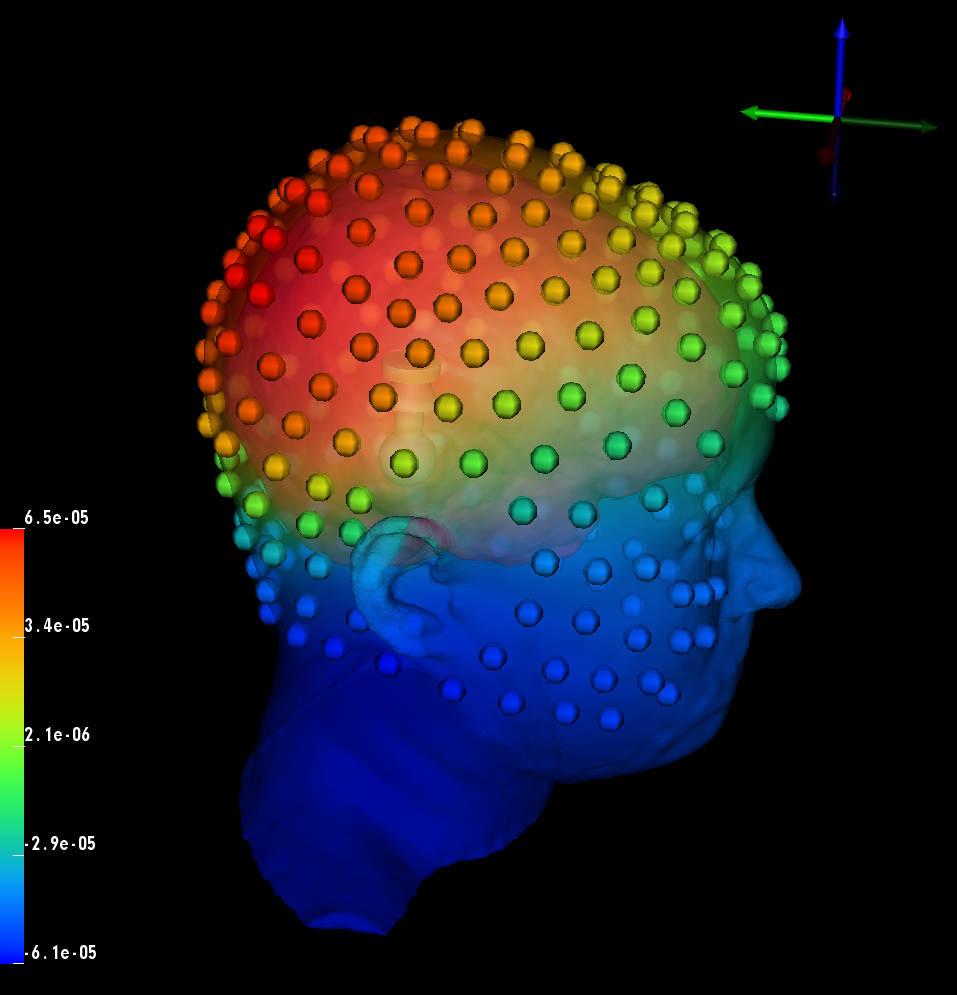
\includegraphics[width=.49\textwidth]{Figures/iso_dipole}
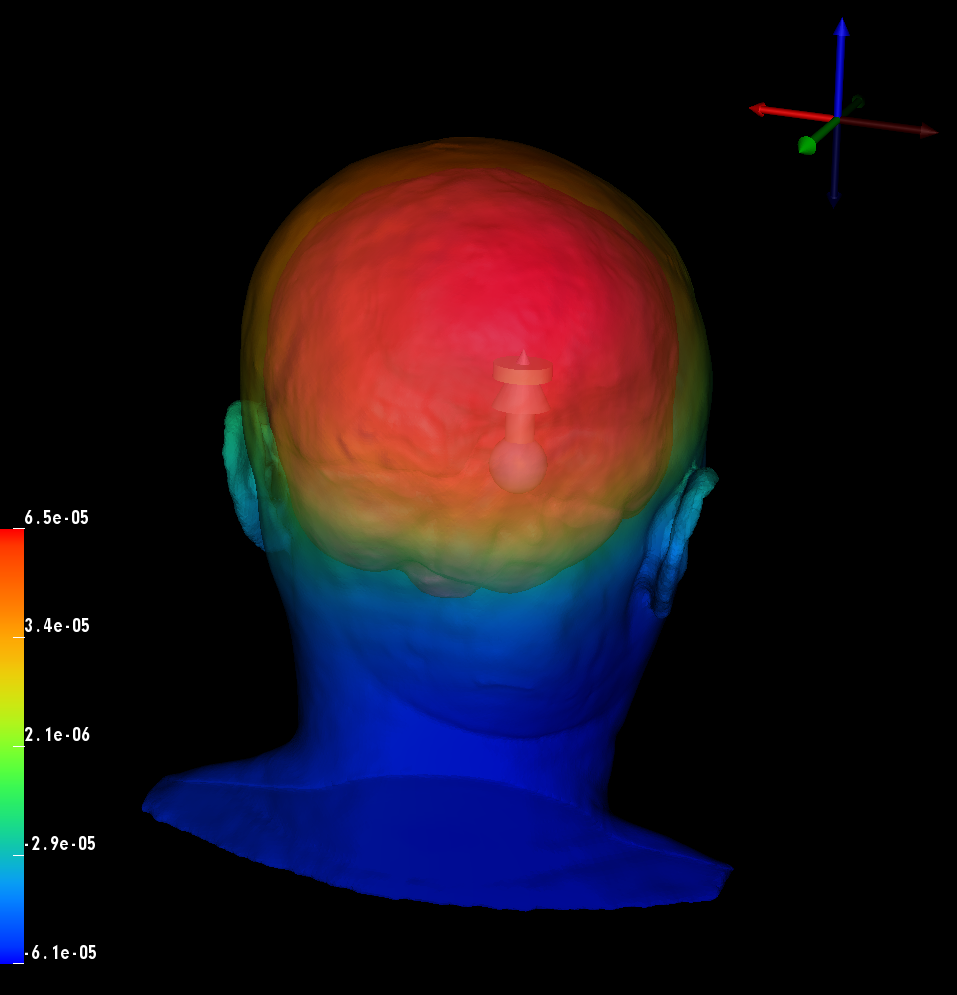
\includegraphics[width=.49\textwidth]{Figures/iso_dipole_2}
\caption{Isotropic forward problem solution with dipole source and data mapped onto the head surface and electrodes.}
\label{fig:isodip}
\end{center}
\end{figure}

\begin{figure}[H]
\begin{center}
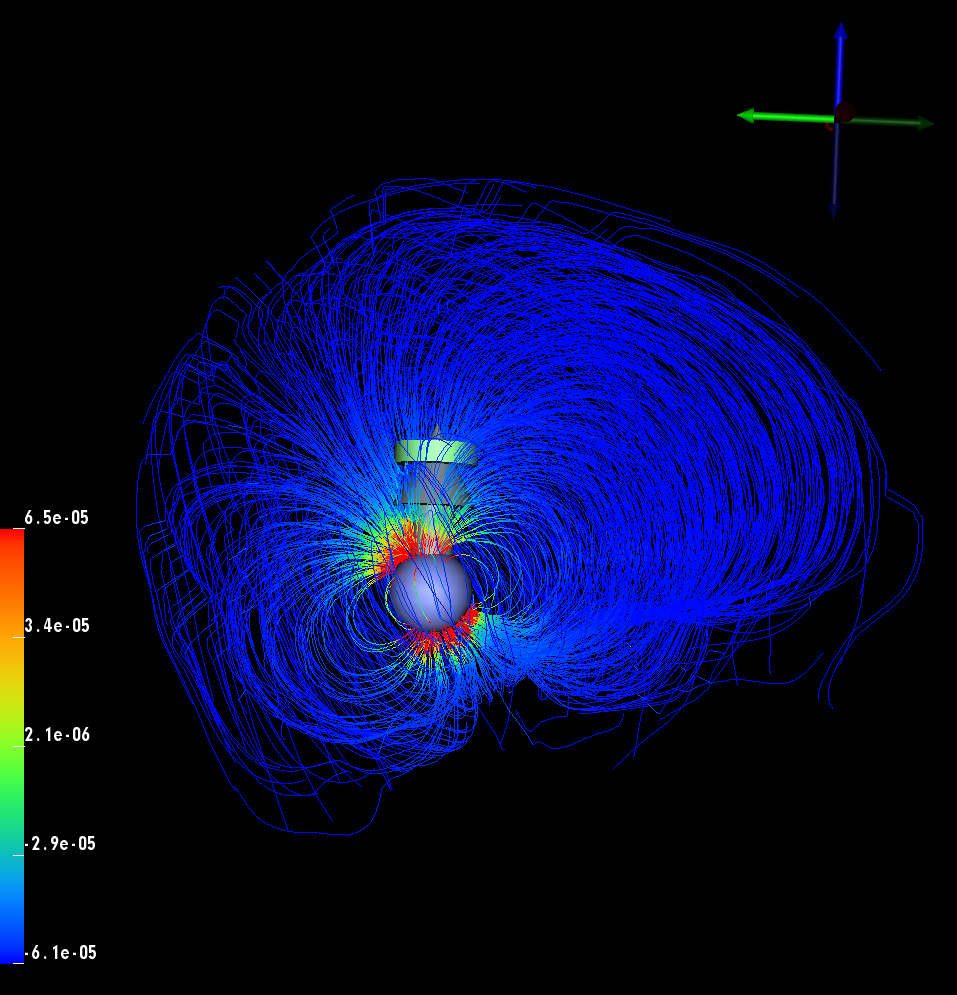
\includegraphics[width=.49\textwidth]{Figures/iso_streamlines}
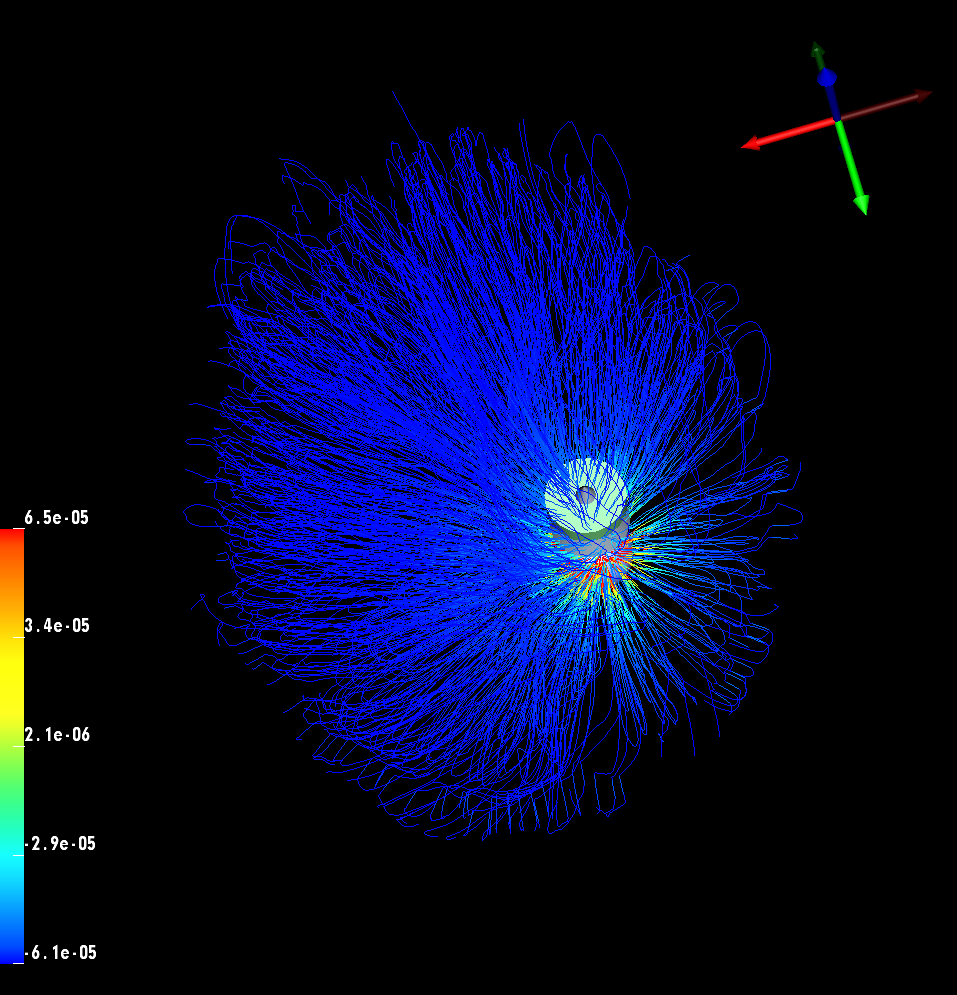
\includegraphics[width=.49\textwidth]{Figures/iso_streamlines_top}
\caption{Isotropic streamlines visualization with dipole source made in SCIRun}
\label{fig:isostream}
\end{center}
\end{figure}

\subsubsection{Anisotropic}

An anisotropic, inhomogeneous head model is expected to not have spherical results. This can be seen with streamlines, and even more so with isolines. As discussed in \ref{sec:cond}, there are two methods of scaling diffusion tensor data. The network has the option to choose one or the other. The electrodes, the dipoles, and the mesh registered well to the diffusion tensor space.

\begin{figure}[H]
\begin{center}
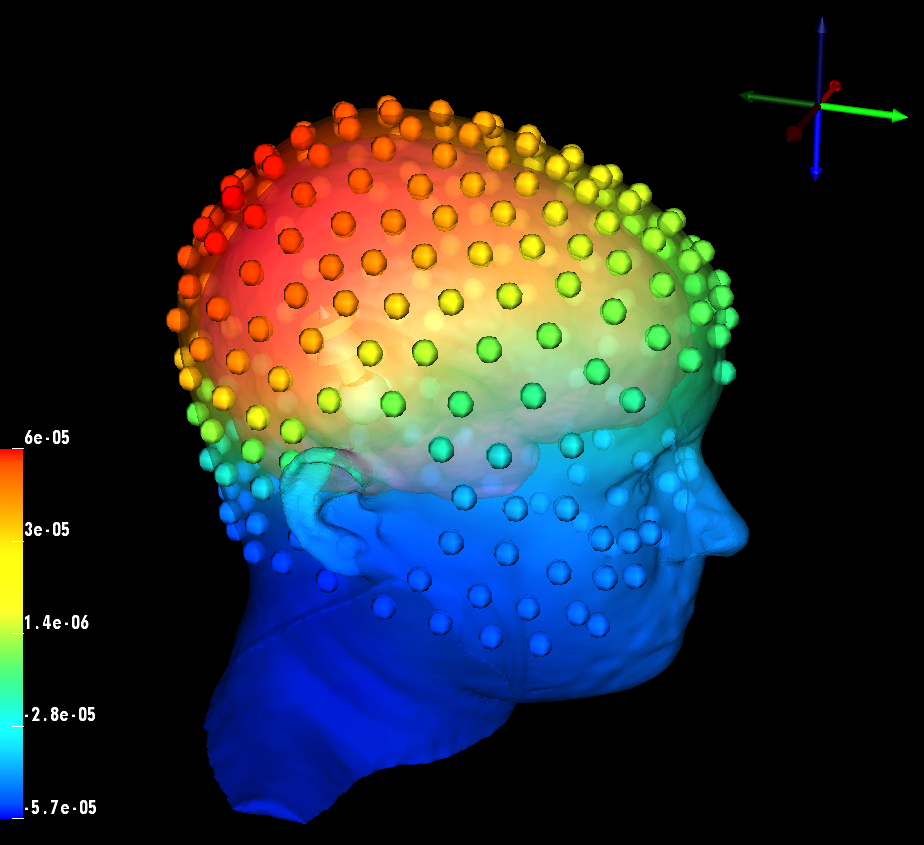
\includegraphics[width=.49\textwidth]{Figures/aniso_dipole}
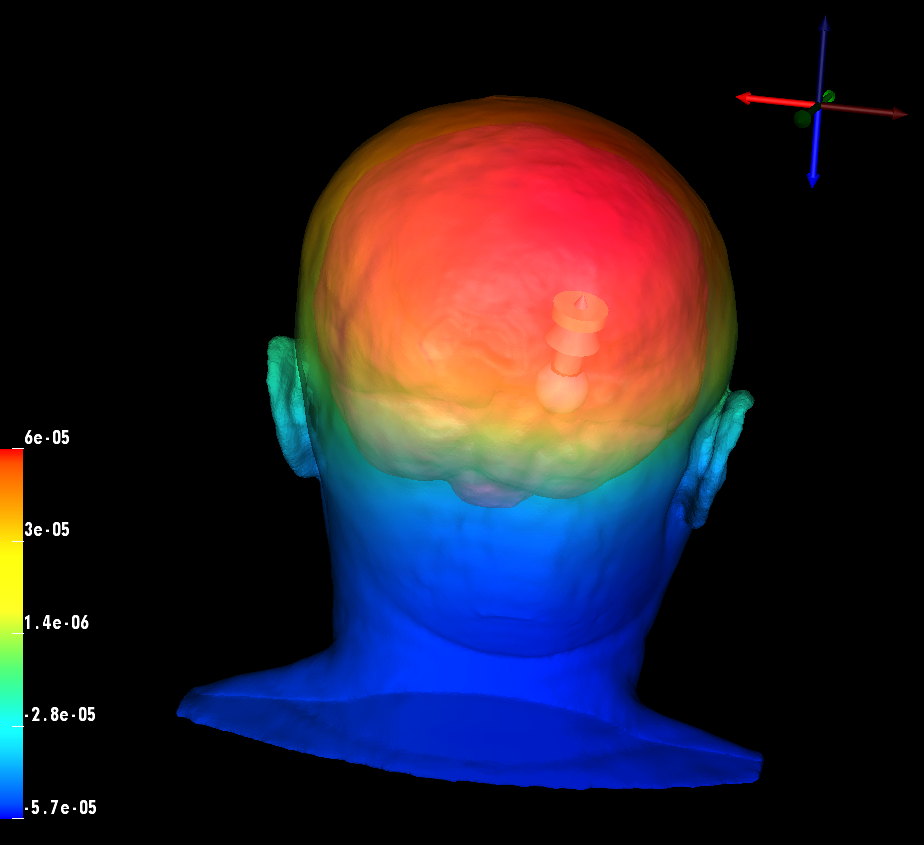
\includegraphics[width=.49\textwidth]{Figures/aniso_dipole_2}
\caption{Anisotropic forward problem solution with dipole source and data mapped onto the head surface and electrodes}
\label{fig:anisodip}
\end{center}
\end{figure}

\begin{figure}[H]
\begin{center}
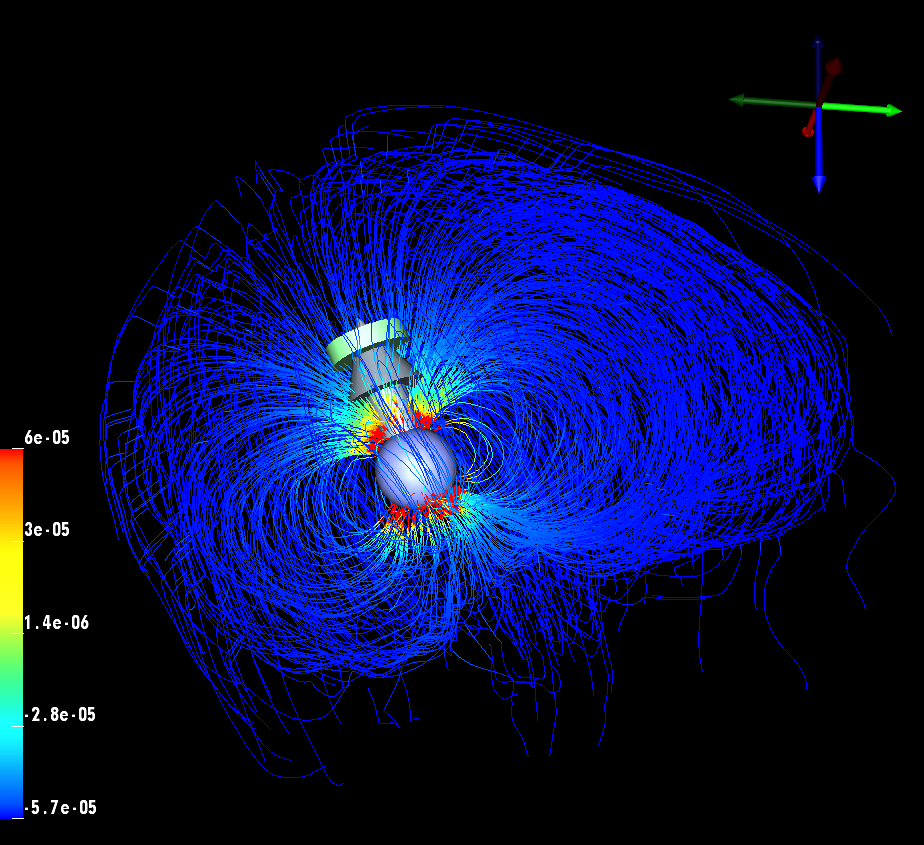
\includegraphics[width=.49\textwidth]{Figures/aniso_streamlines}
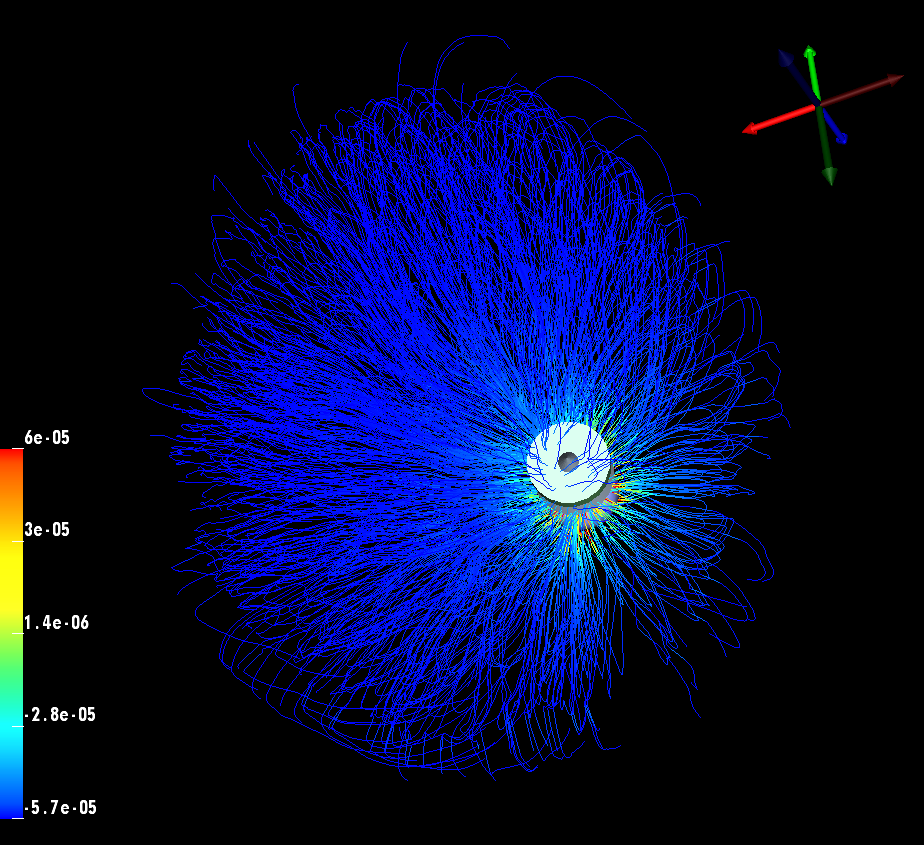
\includegraphics[width=.49\textwidth]{Figures/aniso_streamlines_top}
\caption{Anisotropic streamlines visualization with dipole source made in SCIRun}
\label{fig:anisostream}
\end{center}
\end{figure}

\begin{figure}[H]
\begin{center}
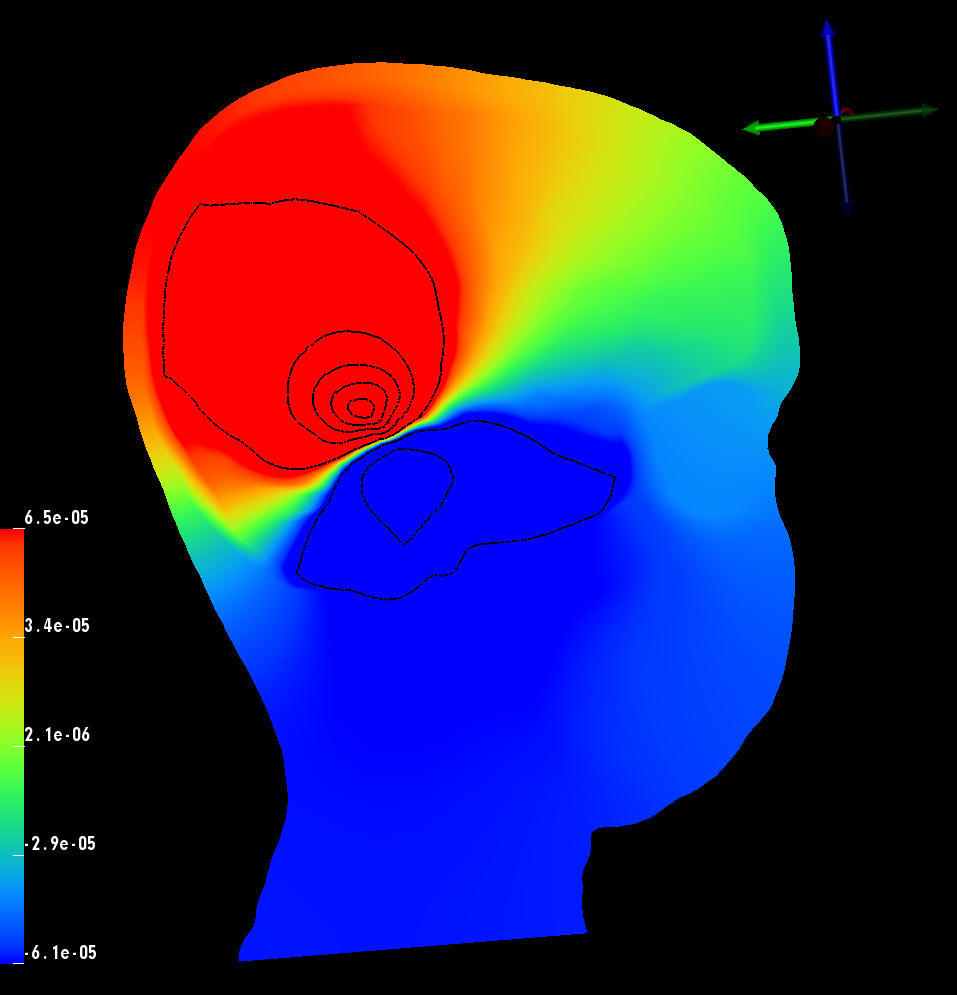
\includegraphics[width=.49\textwidth]{Figures/iso_isolines}
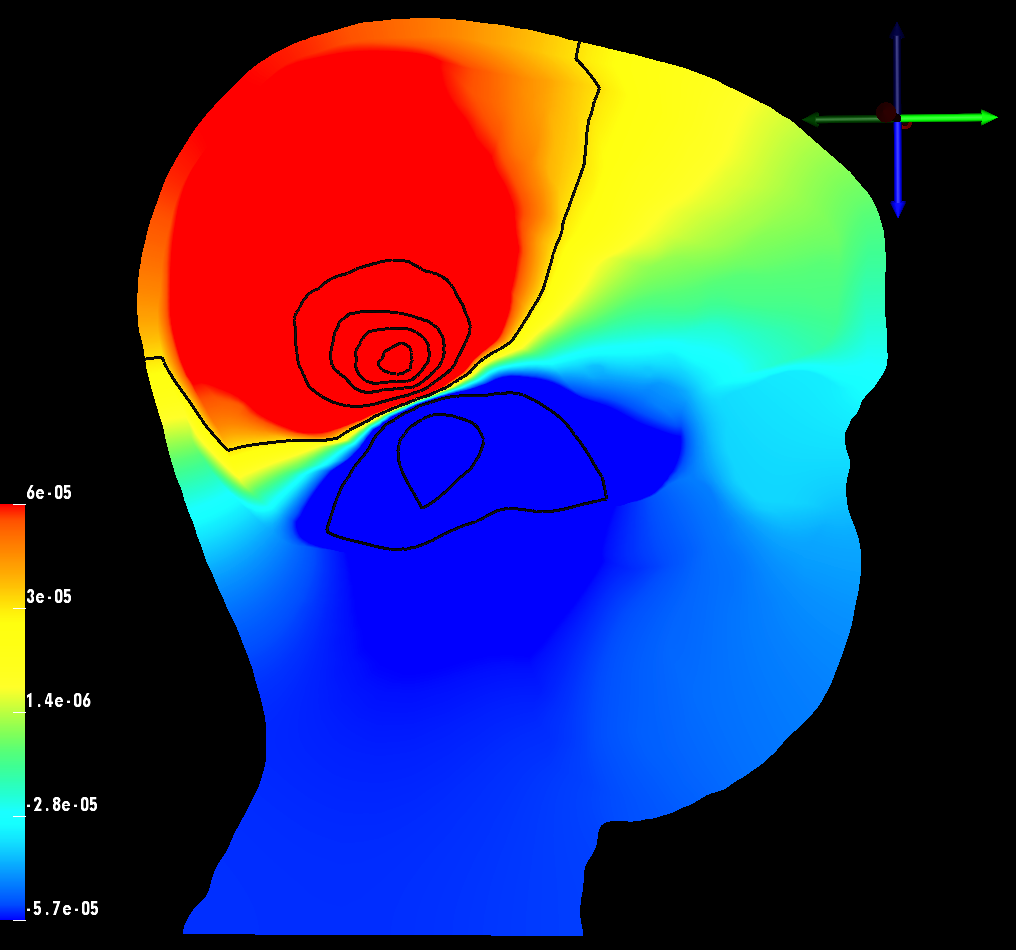
\includegraphics[width = .49\textwidth]{Figures/aniso_isolines}
\caption{Isolines comparison using SCIRun: isotropic white matter conductivity \textit{(left)}, anisotropic white matter conductivity \textit{(right)}}
\label{fig:isolines}
\end{center}
\end{figure}

\subsection{fMRI Visualization}

fMRI data is a novel datatype for SCIRun. With a rigid and manual registration to the mesh coordinate space, the fMRI data was mapped effectively onto the mesh's cortical surface and visualized, which allows for future use of fMRI data in simulations using the SCIRun software package.

\begin{figure}[H]
\begin{center}
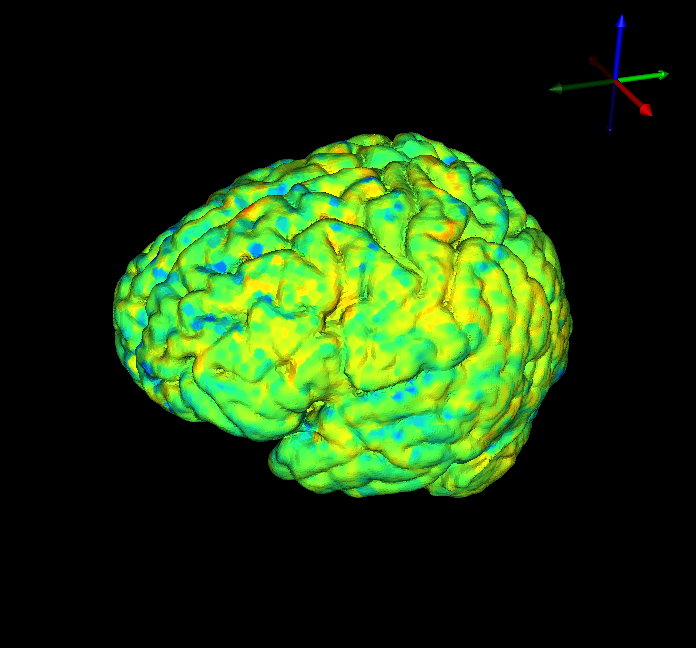
\includegraphics[width=.75\textwidth]{Figures/fmri_1}
\caption{fMRI data visualization in SCIRun: fMRI manual registration \textit{(left)} and fMRI data mapped onto cortical surface mesh \textit{(right)}}
\label{fig:fmrivis}
\end{center}
\end{figure}

\subsection{EEG Visualization}

When using EEG data, the particular application dictates what kind of additional processing, filtering, and cutting of the data needs to be done. There are bad leads in these visualizations, specifically around the eyes, possibly due to blinking or eyes rolling. The bad leads will be remedied with further specific processing.

\begin{figure}[H]
\begin{center}
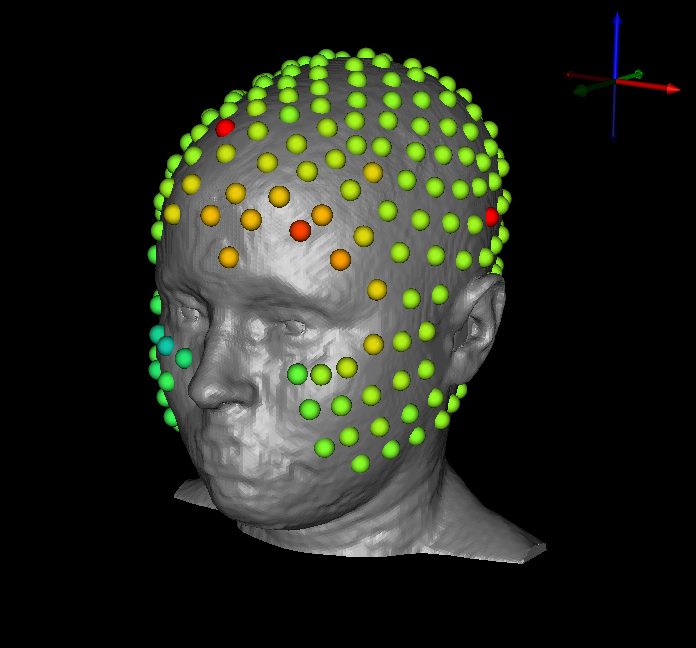
\includegraphics[width=.49\textwidth]{Figures/eeg_1}
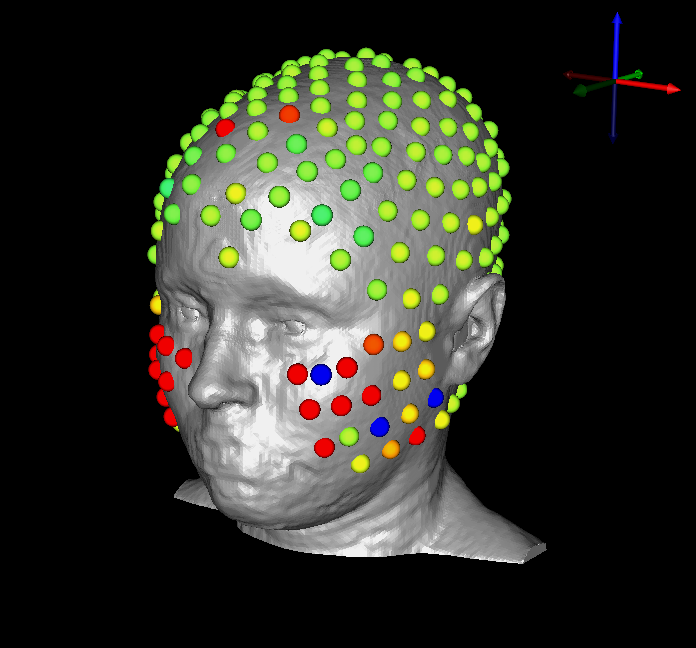
\includegraphics[width=.49\textwidth]{Figures/eeg_2}
\caption{EEG signal visualization using SCIRun. These are examples of ``bad" leads that would need further processing for specific applications}
\label{fig:eegvis}
\end{center}
\end{figure}